\subsection{Grössenvergleiche von unendlichen Mengen}



\begin{definition}{Endlichkeit und Abzählbarkeit}
\begin{itemize}
\item Eine Menge $X$ heisst \textit{endlich}, falls $X=\varnothing$ oder eine natürliche Zahl $n\geq 1$ und eine bijektive Funktion $f:X \to \{1,\dots,n\}$ existieren.
Ist $X\neq\varnothing$ eine endliche Menge, dann existiert eine Darstellung der Form $X=\{x_1,x_2,\dots,x_n\}$ wobei die Elemente $x_i$ paarweise verschieden sind (d.h. es gilt $i\neq j\Rightarrow x_i\neq x_j$). In diesem Fall hat die Menge $X$ genau $n$ viele Elemente und wir schreiben $|X|=n$. Weiter schreiben wir $|\varnothing| = 0$.
\item Nicht endliche Mengen nennen wir \textit{unendlich}.
\item Eine Menge $X$ heisst \textit{abzählbar}, wenn eine surjektive Funktion $F:\N\to X$ existiert oder wenn $X=\varnothing$ gilt.
\item Die Menge $X$ heisst \textit{abzählbar unendlich}, wenn $X$ abzählbar und unendlich ist.
\item Eine \textit{überabzählbare} Menge ist eine Menge, die nicht abzählbar ist.
\end{itemize}
\end{definition}
\begin{comment}
\begin{remark}\label{rk:abzMengeAnschauung}
Ähnlich wie im Fall von endlichen Mengen ist jede nichtleere abzählbare Menge $X$ von der Form
\[
X=\{a_0,a_1,a_2,\dots \}=\{a_i\mid i\in\N\}.
\]
Den Zusammenhang zu Definition von Endlichkeit und Abzählbarkeit liefert hier die Funktion $F:\N\to X$, die durch $F(i)=a_i$ gegeben ist.
\end{remark}

\begin{remark}
Abzählbare Mengen kann man sich auch als die Mengen vorstellen, deren Elemente von den natürlichen Zahlen durchnummeriert  (Wiederholungen erlaubt) werden können. Die Elemente einer abzählbaren Menge lassen sich also in eine Liste schreiben, die für jede natürliche Zahl eine Zeile hat.
\begin{center}
\begin{tabular}{c|c}
$\N$ & $X$\\
\hline
$0$ & $x$\\
$1$ & $y$\\
$2$ & $z$\\
$\vdots$ & $\vdots$
\end{tabular}
\end{center}
\end{remark}
\end{comment}

\begin{lemma}{Schubfachprinzip}
    Wenn $n$ Objekte auf $m$ Behälter verteilt werden und $n>m$ gilt, dann gibt es mindestens einen Behälter, der mehr als ein Objekt enthält. Formal, sind $n>m$ natürliche Zahlen und gelte $|X|= n$ sowie $|Y|=m$, dann gibt es keine injektive Funktion
    \begin{align*}
    F: X\to Y.
    \end{align*}
\end{lemma}

\begin{lemma}{Injektive Abbildung der natürlichen Zahlen}\\
    Gibt es eine injektive Funktion $F:\N\to A$, dann ist die Menge $A$ unendlich.
\end{lemma}

\begin{proof}{Unendlichkeit zeigen}
    Es sei eine Menge $A$ und eine injektive Funktion $F:\N\to A$ gegeben. Wäre die Menge $A$ endlich, dann gäbe es eine natürliche Zahl $n$ mit $|A|=n$. Die Funktion
    \begin{align*}
    G&:\{0,\dots,n\}\to A\\
    G&(x) = F(x)
    \end{align*}
    wäre injektiv und würde, wegen $|\{0,\dots,n\}|=n+1$, dem Schubfachprinzip widersprechen.
\end{proof}

\begin{lemma}{Abzählbare Mengen}
    Folgende Aussagen sind für unendliche Mengen $A$ äquivalent:
    \begin{enumerate}
        \item Die Menge $A$ ist abzählbar.
        \item Es gibt eine surjektive Funktion $F_{\N,A}:\N\to A$.
        \item Es gibt eine injektive Funktion $F_{A,\N}:A\to\N$.
        \item Es gibt eine bijektive Funktion $B_{\N,A}:\N\to A$.
        \item Es gibt eine bijektive Funktion $B_{A,\N}:A\to\N$.
    \end{enumerate}
\end{lemma}

\begin{proof}{Abzählbarkeit mit Funktionen zeigen}
    \begin{itemize}
        \item Die Aussagen in $a)$ und $b)$ sind per Definition äquivalent.
        \item Die Aussagen in $d)$ und $e)$ sind offensichtlich äquivalent (Umkehrfunktion).
        %\item Für die Implikation $b)\Rightarrow c)$ definieren wir
        %\begin{align*}
        %    F_{A,\N}(a)=\min\{n\in\N \mid F_{\N,A}(n)=a\},
        %\end{align*}
        %dies ist gerechtfertigt\footnote{Wir gehen hier davon aus, dass jede nichtleere Menge von natürlichen Zahlen ein kleinstes Element besitzt, eine Tatsache die wir später beweisen werden.}, da aus der Surjektivität von $F_{\N,A}:\N\to A$ folgt, dass zu jedem $a\in A$ mindestens ein $n\in\N$ mit $F_{\N,A}(n)=a$ existiert. Es bleibt die Injektivität von $F_{A,\N}$ nachzuweisen, dazu nehmen wir $F_{A,\N}(a)=F_{A,\N}(a')$ an. Es folgt, dass es eine natürliche Zahl $n$ mit $F_{\N,A}(n)=a$ und $F_{\N,A}(n)=a'$ gibt. Somit muss wie gewünscht $a=a'$ gelten.
        \item Für die Implikation $c)\Rightarrow b)$, gehen wir von einer injektiven Funktion $F_{A,\N}:A\to\N$ aus.
        Weil diese Funktion injektiv ist, und weil $Dom(F_{A,\N})=A$ gilt, ist
        \begin{align*}
            F_{A,\N}^{-1}:Im(F_{A,\N}) \to A
        \end{align*}
        eine surjektive Funktion. Um eine surjektive Funktion von $\N$ nach $A$ zu erhalten, brauchen wir bloss noch die ``restlichen'' Elemente aus $\N$ zuzuordnen, dazu wählen wir ein beliebiges Element aus $a\in A$ und setzen:
        \begin{align*}
            F_{\N,A}(n)=
                \begin{cases}
                F_{A,\N}^{-1}(n)&\text{falls }n\in Im(F_{A,\N})\\
                a&\text{sonst}
                \end{cases}
        \end{align*}
        \item Für die Implikation $b)\Rightarrow d)$ müssen wir, ausgehend von einer unendlichen Menge $A$ und einer surjektiven Abbildung $F_{\N,A}: \N\to A$, eine bijektive Abbildung $B_{\N,A}: \N\to A$ konstruieren. Da uns für einen vollständigen Beweis die Werkzeuge noch fehlen (Rekursion), wollen wir hier bloss eine Beweisskizze präsentieren. Wir definieren die Funktion $B_{\N,A}$ rekursiv wie folgt:
        \begin{align*}
        B_{\N,A}(0) &= F_{\N,A}(0)\\
        B_{\N,A}(n+1) &= F_{\N,A}(\min\{k\in\N\mid F(k)\neq B_{\N,A}(0),\dots,B_{\N,A}(n) \})
        \end{align*}
        Die resultierende Funktion ist auf ganz $\N$ definiert, weil die Menge $A$ unendlich ist (würde die Rekursion abbrechen, dann wäre $A$ von der Form $\{F_{\N,A}(0),\dots,F_{\N,A}(m)\}$ für ein $m\in\N$). Die Funktion $B_{\N,A}$ ist surjektiv, weil $F_{\N,A}$ surjektiv ist. Die Injektivität folgt, weil per Konstruktion für alle $x,y$
        \begin{align*}
        x<y \Rightarrow B_{\N,A}(x) \neq B_{\N,A}(y)
        \end{align*}
        gilt.
    \end{itemize}
    Weil aus $d)$ und $e)$ alle anderen Aussagen direkt folgen, genügen die gezeigten Implikationen für den Beweis des Satzes.
\end{proof}



\begin{lemma}{Endliche Mengen}
Jede endliche Menge ist abzählbar.
\end{lemma}

\begin{proof}{Abzählbarkeit endlicher Mengen}
Ist $X$ eine endliche Menge, dann können wir $X$ als $\{x_1,\dots,x_n\}$ mit einer natürlichen Zahl $n$ schreiben. Da die leere Menge per Definition abzählbar ist, können wir annehmen, dass $X$ mindestens ein Element $x_1$ besitzt. Wir definieren nun die Funktion $F:\N\to X$ mit
\begin{align*}
F(i)=\begin{cases}
x_i&\text{falls }0<i\leq n\\
x_1&\text{sonst.}
\end{cases}
\end{align*}
Da $F$ offensichtlich jedes Element von $X=\{x_1\dots x_n\}$ trifft, ist $F$ surjektiv. Somit ist $X$ abzählbar.
\end{proof}

\begin{lemma}{Teilmengen}
Jede Teilmenge einer abzählbaren Menge ist abzählbar.
\end{lemma}
\begin{proof}{Abzählbarkeit Teilmengen}
Es sei $X\subseteq Y$ und $Y$ sei eine abzählbare Menge. Da $Y$ abzählbar ist,
gibt es eine surjektive Funktion $F:\N\to Y$. Wenn $X=\varnothing$ gilt, dann
ist $X$ per Definition abzählbar und wir sind fertig. Ist $X\neq\varnothing$,
dann gibt es ein Element $a\in X$. Wir können nun wie folgt eine Abbildung
$G:\N\to X$ angeben.
\begin{align*}
G(x)=\begin{cases}
F(x)&\text{falls }F(x)\in X\\
a&\text{sonst.}
\end{cases}
\end{align*}
Da $X\subseteq Y$ gilt und weil jedes Element von $Y$ von der Funktion $F$
getroffen wird, wird auch jedes Element von $X$ von $G$ getroffen. Somit
ist $G:\N\to X$ surjektiv und $X$ ist also abzählbar.
\end{proof}

\begin{lemma}{Transitivität}
Ist $X$ eine abzählbare Menge und gibt es eine surjektive Funktion $F:X\to Y$, dann ist auch $Y$ abzählbar.
\end{lemma}
\begin{proof}{Abzählbarkeit Transitivität}
Diese Behauptung folgt sofort aus den Regeln der Komposition (die Komposition von surjektiven Funktionen ist wieder surjektiv).
%Sollte $X$ die leere Menge sein, dann ist auch $Y$ leer und somit abzählbar. Ist $X$ nichtleer, dann folgt aus der Abzählbarkeit von $X$, dass es eine surjektive Abbildung $G:\N\to X$ gibt. Wir können nun die Funktion $H:\N\to Y$ durch Komposition der Funktionen $F$ und $G$ bilden, d.h. wir definieren
%\begin{align*}
%H:\N\to Y\phantom{abstand}\text{ mit }\phantom{abstand} H(n)=F(G(n)).
%\end{align*}
%Wir müssen nun noch zeigen, dass wir mit der Funktion $H$ jedes Element von $Y$ treffen. Wir nehmen dazu ein beliebiges Element $y$ von $Y$ und zeigen, dass es eine natürliche Zahl $n$ gibt mit $H(n)=y$. Es sei also $y\in Y$ beliebig. Da die Funktion $F:X\to Y$ surjektiv ist, muss es ein $x\in X$ geben so, dass $F(x)=y$ gilt. Weil aber auch die Funktion $G:\N\to X$ surjektiv ist, muss es ebenfalls eine natürliche Zahl $n$ geben, mit $G(n)=x$. Zusammenfassend können wir also sagen, dass es eine natürliche Zahl und ein Element $x$ aus $X$ gibt, mit der Eigenschaft
%\[
%H(n)=F(G(n))=F(x)=y.
%\]
%Weil $y\in Y$ beliebig gewählt wurde, ist die Funktion $H$ surjektiv.
\end{proof}



\begin{lemma}{Erstes Diagonalargument Cantor}
Die Menge $\N\times\N$, bestehend aus allen Paaren von natürlichen Zahlen, ist abzählbar.
\end{lemma}
\begin{proof}{Beweisidee Erstes Diagonalargument}
Anstelle eines formalen Beweises, skizzieren wir eine Abzählung aller Paare von natürlichen Zahlen wie folgt:
%\begin{figure}[h!]
\begin{center}
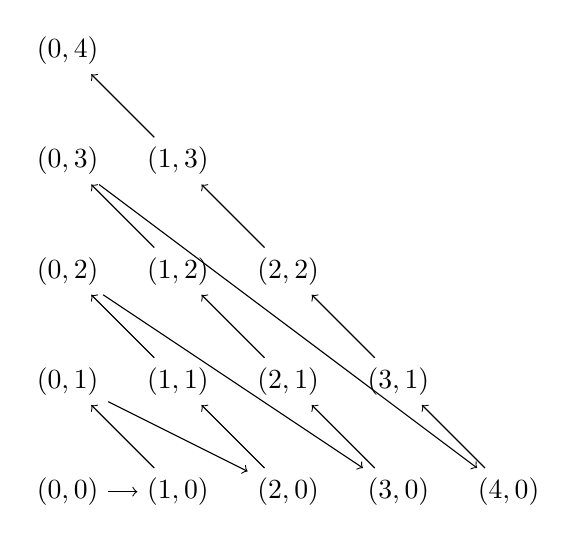
\begin{tikzpicture}[scale=1.4]
\node (0) at (0,0) {$(0,0)$};
\node (2) at (0,1) {$(0,1)$};
\node (5) at (0,2) {$(0,2)$};
\node (9) at (0,3) {$(0,3)$};
\node (14) at (0,4) {$(0,4)$};
\node (1) at (1,0) {$(1,0)$};
\node (4) at (1,1) {$(1,1)$};
\node (8) at (1,2) {$(1,2)$};
\node (13) at (1,3) {$(1,3)$};
\node (3) at (2,0) {$(2,0)$};
\node (7) at (2,1) {$(2,1)$};
\node (12) at (2,2) {$(2,2)$};
\node (6) at (3,0) {$(3,0)$};
\node (11) at (3,1) {$(3,1)$};
\node (10) at (4,0) {$(4,0)$};
\draw[->] (0) -- (1);
\draw[->] (1) -- (2);
\draw[->] (2) -- (3);
\draw[->] (3) -- (4);
\draw[->] (4) -- (5);
\draw[->] (5) -- (6);
\draw[->] (6) -- (7);
\draw[->] (7) -- (8);
\draw[->] (8) -- (9);
\draw[->] (9) -- (10);
\draw[->] (10) -- (11);
\draw[->] (11) -- (12);
\draw[->] (12) -- (13);
\draw[->] (13) -- (14);
\end{tikzpicture}
%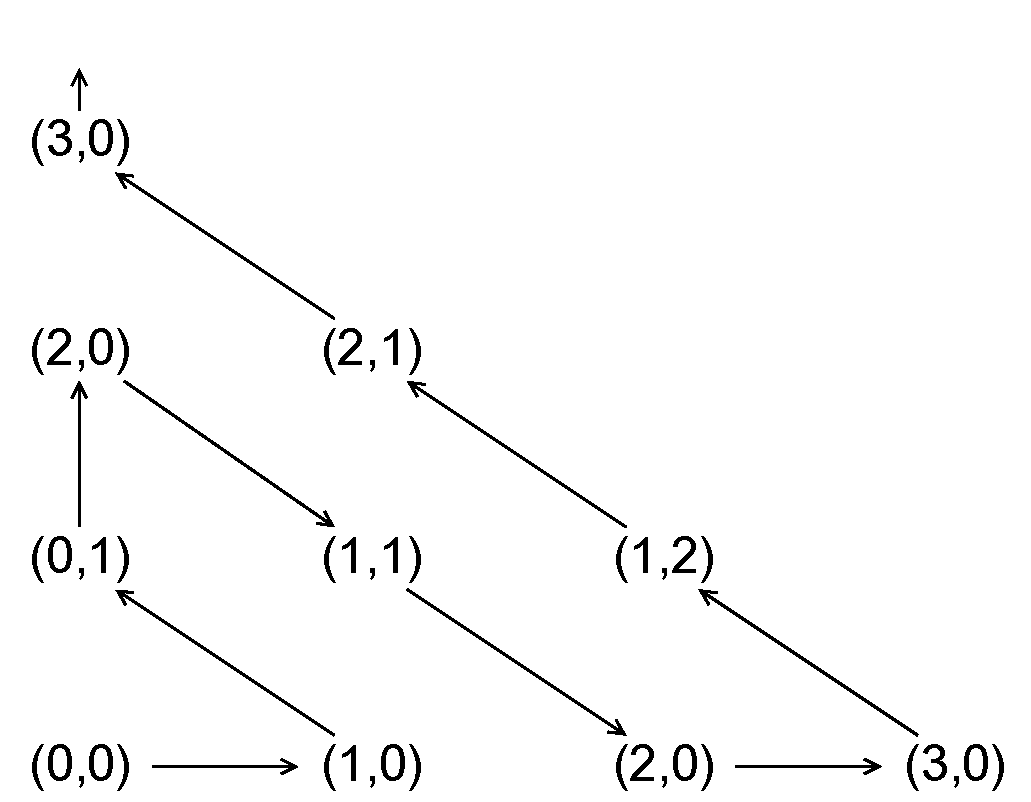
\includegraphics[width=0.5\textwidth]{figures/cantor1}
%\caption*{Die Pfeile deuten die Reihenfolge an, in der die Elemente von $\N\times\N$ abgezählt werden.}
\end{center}
\ %end{figure}
\end{proof}
\begin{lemma}{Vereinigung}
Jede Vereinigung von abzählbar vielen abzählbaren Mengen ist abzählbar. Konkret, jede Vereinigung von der Form
\[
\bigcup_{i\in\N}A_i
\]
ist abzählbar, wenn alle $A_i$'s abzählbar sind.
\end{lemma}
\begin{proof}{Abzählbarkeit Vereinigung}
Wir nehmen an, dass die Menge $\{A_i\mid i\in \N \}$ aus lauter abzählbaren Mengen besteht. Um zu zeigen, dass $\bigcup_{i\in N}A_i$ abzählbar ist, genügt es, aufgrund von Satz~\ref{satz:abzaehlbarTransitiv} und Satz~\ref{cantor1}, zu zeigen, dass es eine surjektive Funktion
\[
H:\N\times\N\to\bigcup_{i\in N}A_i
\]
gibt. Da für jede natürliche Zahl $i$ die Menge $A_i$ abzählbar ist, gibt es für jede natürliche Zahl $i$ auch eine surjektive Funktion $F_i:\N\to A_i$. Wir können die Vereinigungsmenge der $A_i$'s also wie folgt schreiben:
\begin{align*}
\bigcup_{i\in \N}A_i&=\{F_i(j)\mid i,j\in\N \}\\
&=\{F_i(j)\mid (i,j)\in\N\times\N \}.
\end{align*}
Daraus folgt, dass die Funktion
\[
H:\N\times\N\to \bigcup_{i\in N}A_i\phantom{abstand}\text{mit}\phantom{abstand} H(i,j)=F_i(j),
\]
die gesuchte surjektive Funktion ist.
\end{proof}

\begin{corollary}{Kartesisches Produkt}
Die Menge $\Z\times \Z$ ist abzählbar.
\end{corollary}
\begin{proof}{Abzählbarkeit Kartesisches Produkt}
Wir wissen bereits, dass die Menge $\N\times\N$ abzählbar ist. Daraus folgt, dass auch die Mengen
\begin{align*}
X&=\N\times\{-n\mid n\in \N\}\\
Y&=\{-n\mid n\in \N\}\times\N \\
Z&=\{-n\mid n\in \N\}\times\{-n\mid n\in \N\}
\end{align*}
abzählbar sind. Aus Satz~\ref{satz:countableUnion} folgt also, dass die Menge
\[
\Z\times\Z=(\N\times\N)\cup X\cup Y\cup Z
\]
abzählbar ist.
\end{proof}

\begin{corollary}{Rationale Zahlen}
Die Menge $\Q=\big\{\frac{x}{y}\mid x,y\in \Z\big\}$ der rationalen Zahlen (Brüche) ist abzählbar.
\end{corollary}
\begin{proof}{Abzählbarkeit Rationale Zahlen}
Da die Funktion
\[
F:\Z\times(\Z\setminus{\{0\}})\to \Q\phantom{abstand}\text{mit}\phantom{abstand}F(x,y)=\frac{x}{y}
\]
surjektiv ist, folgt die Behauptung aus Satz~\ref{satz:abzaehlbarTransitiv}.
\end{proof}



\begin{theorem}{Zweites Diagonalargument Cantor}
Die Menge aller unendlichen Binärsequenzen (Sequenzen aus Nullen und Einsen) ist überabzählbar.
\end{theorem}
\begin{proof}{Beweis zweites Diagonalargument}
Beweis durch Widerspruch. Wäre die Menge aller unendlichen Binärsequenzen abzählbar, dann gäbe es eine Liste von der Form\footnote{Natürlich ist die angedeutete Liste Beispielhaft und dient nur der Veranschaulichung unserer Konstruktion der Sequenz $b$. Die Sequenz $s_0$, beispielsweise, könnte auch mit dem Präfix $00000100$ oder irgend einer anderen Folge von Nullen und Einsen beginnen. }
\begin{center}
\begin{tabular}{c|l}
$\N$ & Binärsequenzen\\
\hline
$0$ & $s_0=01101011\cdots$\\
$1$ & $s_1=10010110\cdots$\\
$2$ & $s_2=00101001\cdots$\\
$\vdots$ & $\vdots$
\end{tabular}
\end{center}
in der alle unendlichen Binärsequenzen vorkommen. Wir konstruieren nun, ausgehend von dieser Liste, eine Binärsequenz $b$, die nicht in der Liste enthalten sein kann. Wir definieren $b$ wie folgt:
\begin{align*}
0\text{-tes Glied}&=b(0)=1-s_0(0)\\
1\text{-tes Glied}&=b(1)=1-s_1(1)\\
2\text{-tes Glied}&=b(2)=1-s_2(2)\\
&\vdots\\
n\text{-tes Glied}&=b(n)=1-s_n(n)\\
&\vdots
\end{align*}
Die Folge $b=110\cdots$ kann nicht in der Liste vorkommen, weil sie sich von jedem Element in der Liste in mindestens einem Glied unterscheidet (von der $n$-ten Sequenz unterscheidet sich $b$ im $n$-ten Glied). Dies steht im Widerspruch zu unserer Annahme, dass in der Liste alle unendlichen Binärsequenzen vorkommen.
\end{proof}


\begin{corollary}{Intervall}
Das Intervall $(0,1)=\{r\in\R\mid 0<r<1 \}$ ist überabzählbar. Insbesondere ist die Menge $\R$ der reellen Zahlen überabzählbar.
\end{corollary}
\begin{proof}{Überabzählbarkeit Intervall}
Die reellen Zahlen (in Binärdarstellung) im Intervall $(0,1)$, sind von der Form $0,\dots$ wobei $\dots$ für eine unendliche Binärsequenz steht. Daher steht das Intervall $(0,1)$ mit der Menge aller unendlichen Binärsequenzen in eins-zu-eins Korrespondenz. Die Behauptung folgt daher aus Theorem~\ref{thrm:cantor2}.
\end{proof}

\begin{corollary}{Potenzmenge}
Die Potenzmenge von $\N$ ist überabzählbar.
\end{corollary}
\begin{proof}{Überabzählbarkeit Potenzmenge}
Jede Teilmenge $A$ von $\N$ kann wie folgt durch eine Binärsequenz $\chi_A$ beschrieben werden:
\begin{align*}
\chi_A(n)=\begin{cases}
1&\text{falls } n\in A\\
0&\text{falls} n\notin A.
\end{cases}
\end{align*}
Daher folgt die Behauptung aus Theorem~\ref{thrm:cantor2}.
\end{proof}

\begin{corollary}{Menge aller Funktionen}
Die Menge aller Funktionen $F:\N\to\N$ ist überabzählbar.
\end{corollary}
\begin{proof}{Überabzählbarkeit der Menge aller Funktionen}
Die Menge der Binärsequenzen entspricht der Menge der Funktionen $F:\N\to\{0,1\}$. Daher folgt die Behauptung aus Theorem~\ref{thrm:cantor2}.
\end{proof}

\begin{corollary}{Unberechenbare Funktionen}
Es gibt Funktionen $F:\N\to\N$, die von keinem Java, C, C++, Fortran\dots Programm berechenbar sind. Solche Funktionen heissen \textit{unberechenbar}.
\end{corollary}



